%نام و نام خانوادگی:
%شماره دانشجویی: 
\مسئله{}
پیدا کردن نیازمندی‌های غیرکارکردی یکی فعالیت‌هایی است که در مرحله شناسایی نیازمندی‌ها انجام می‌شود.

\begin{enumerate}[a)]
	\item 
	 نیازمندی‌های غیر کارکردی را تعریف کنید و اهمیت آن‌ها را برای یک سیستم نرم‌افزاری تشریح کنید.
	 
	 \item 
	 تحقیق کنید که در متدولوژی‌های چابک چگونه نیازمندی‌های غیرکارکردی را شناسایی و چگونه آن‌ها را در فرآیند محقق می‌کنند.
\end{enumerate}


\پاسخ{

\begin{enumerate}[a)]
	\item
نیازمندی‌های غیرکارکردی را می‌توان تحت عنوان جنبه‌های کیفی، کارآیی، امنیتی و محدودیت‌های عمومی روی یک سیستم تعریف کرد. مشخص کردن این نوع نیازمندی‌ها عموما برای ذی‌نفعان کار آسانی نیست. همچنین در حالی که در تصور کلی، تمرکز بیش‌تری روی کارکرد یک سیستم وجود دارد، عموما این کارکردها بدون توجه به ویژگی‌های غیرکارکردی قابل استفاده نیستند \cite{1-1}.

با این وجود باید توجه کرد که تعریف‌های بسیار زیادی در مورد نیازمندی‌های غیرکارکردی در منابع گوناگون ذکر شده است. برخی از آن‌ها در زیر آورده شده است:

\begin{enumerate}[1-]
	\item
	 نیازمندی‌های غیرکارکردی خواص غیررفتاری یک سیستم را توصیف کرده و بیانگیر ویژگی‌ها و محدودیت‌هایی هستند که سیستم باید با توجه به آن‌ها کار کند \cite{Anton}.
	\item
	 نیازمندی‌های غیرکارکردی، ویژگی‌های کلی یک سیستم شامل قابلیت پورت‌کردن، اتکاپذیری، کاراایی، مهندسی انسانی، تست‌پذیری، قابل‌فهم بودن و تغییر‌پذیر بودن هستند \cite{davis}.
	
	\item 
	نیازمندی غیرکارکردی به نیازمندی‌‌ای گویند که یکی از خواص سیستم را مشخص می‌کند، نظیر محدودیت‌های محیطی یا پیاده‌سازی، کارایی، وابستگی‌های پلتفرمی، قابلیت نگه‌داشت، قابلیتت گسترش و قابلیت اتکا. به بیان دیگر، نیازمندی‌هایی که یک محدودیت را روی نیازمندی‌های کارکردی سیستم مشخص می‌کنند \cite{Rumbaugh}.
	
	\item 
	نیازمندی‌های غیرکارکردی، خواص رفتاری‌ای هستند که کارکردهای مشخص شده باید داشته باند. نظیر قابلیت استفاده یا کارایی \cite{Ncube}.
	
	\item 
	نیازمندی‌های غیرکارکردی توصیفی از یک ویژگی یا مشخصه هستند که یک سیستم نرم‌افزاری باید داشته باشد. به بیان دیگر، محدودیت‌هایی که یک نرم‌افزار فارغ از رفتار قابل مشاهده سیستم باید از آن‌ها پیروی‌ کند \cite{wiegers}.
	
	\item 
	لغت نیازمندی‌های غیرکارکردی برای توصیف نیازمندی‌هایی استفاده می‌شد که متمرکز بر این هستند که یک نرم‌افزار «چقدر خوب» کاری را انجام می‌دهد؛ در مقابلِ نیازمندی‌های کارکردی که متمرکز بر این هستند که نرم‌افزار «چه چیزی» را انجام می دهد \cite{refqs}.

	
\end{enumerate}

مفهوم کیفیت، مفهومی اساسی و بنیادین در مهندسی نرم‌افزار است و در هنگام تولید یک نرم‌افزار باکیفیت، باید هم نیازمندی‌های کارکردی و هم نیازمندی‌های غیرکارکردی مورد توجه قرار بگیرند. با این وجود به دلایل مختلفی نظیر تقاضا برای ساخت نسخه اولیه نرم‌افزار برای نشان دادن به مشتری و همچنین به دلیل ماهیت «نرم» (\lr{Soft})، این نوع نیازمندی‌ها کمتر مورد توجه قرار می‌گیرند \cite{chung}.
	
	به دلیل همین موضوع، خیلی از اوقات تمرکز اصلی برروی طراحی پرجزییات و تست سیستم پیاده‌سازی شده معطوف می‌شود، در حالی که این مراحل بدون توجه و درک مسئله‌ای که این نرم‌افزار برای حل آن در دنیای واقعی ایجاد شده است، بی‌فایده هستند. بسیاری از مسائل دنیای واقعی بیش‌ از آن‌ که وابسته به نیازمندی‌های کارکردی نرم‌افزار باشند، وابسته به نیازمندی‌های غیرکارکردی آن هستند. مواردی نظیر سرعت پردازش، امنیت، راحتی کار با نرم‌افزار، همگی مواردی هستند که تحت عنوان نیازمندی‌های کارکردی قرار نمی‌گیرند اما در صورت محقق نشدن، مشتری ناراضی خواهد بود \cite{chung}.
	
	دسته‌بندی‌های زیادی برای این دسته از نیازمندی‌ها وجود دارد ولی در این جا، ما مطابق استاندارد \lr{ISO25010} تعدادی از نیازمندی‌های غیروظیفه‌ای را ذکر می‌کنیم تا به شکل واضح‌تری با مفهوم نیازمندی‌های غیرکارکردی آشنا شویم \cite{iso25010}.
	
	\begin{itemize}
		\item 
		بهره‌وری عملکرد (\lr{Performance Efficiency})
		
		\begin{itemize}
			\item
			ظرفیت (\lr{Capacity}): ظرفیت به معنی حدی از پارامترهای سیستم است که در آن می‌توانیم نیازمندی‌های کاربر را برطرف کنیم.
			
			\item 
			رفتار زمانی (\lr{Time Behaviour} ): رفتار زمانی به معنی حد مناسب برای مواردی نظیر نرخ گذردهی، سرعت پاسخ دادن و سرعت پردازش است.
			
		\end{itemize}
		
		\item
		سازگاری (\lr{Compatibility})
		\begin{itemize}
			\item
			قابلیت همکاری (\lr{Interoperability}): این خصیصه به معنی این است که دو یا چند سیستم، محصول یا زیر‌سیستم بتوانند به خوبی اطلاعات را با یکدیگر رد و بدل کرده و از آن استفاده کنند.
			
		\end{itemize}
		
		\item
		قابلیت استفاده (\lr{Usability})
		
		\begin{itemize}
			
			\item 
			قابلیت یادگیری (\lr{Learnability}): این خصیصه بیانگر این است که کاربر چقدر راحت می‌تواند کار با سیستم را به شکل بهینه، کارا، بدون نگرانی و با رضایت یاد بگیرد. برای تحقق این مورد، باید رابط کاربری و تجربه کاربری سیستم به شکلی مناسب و تا حد امکان ساده طراحی بشود. همچنین از طریق مستندات آموزشی، نحوه کارکرد سیستم در مواردی که ممکن است ابهام داشته باشند، به کاربر آموزش داده خواهد شد.
			
			\item
			محافظت در مقابل خطاهای کاربر (\lr{User Error Protection}): این مورد به معنی این است که محصول باید طوری طراحی شود که از کاربر در مقابل خطاهایی که ممکن است خود کاربر مرتکب شود محافظت کند. این کار با بررسی دقیق تک تک پروسه‌های سیستم و تشخیص تمامی روندهای ممکن برای هر بخش و پیش‌بینی پیام‌های مناسب برای آن‌ها قابل دستیابی است.
			
			\item 
			دسترس‌پذیری (\lr{Accessibility}): دسترس‌‌پذیری به معنی این است که کاربران با سطح توانایی‌های مختلف (مثلا افرادی که دچار مشکلات بینایی هستند و...) بتوانند به خوبی از سیستم استفاده کنند.
			
			
			\item 
			زیبایی رابط کاربری (\lr{User Interface Aesthetics}): رابط کاربری باید به گونه‌ای طراحی شود که عموم کاربران بتوانند به خوبی با آن تعامل کرده و از کار با آن لذت ببرند. 
			
			
		\end{itemize}
		
		
		\item
		قابلیت اطمینان (\lr{Reliability})
		
		\begin{itemize}
			\item 
			
			در دسترس بودن (\lr{Availability}): به معنی در دسترس و عملیاتی بودن سیستم در زمان‌های لازم است.
			
			\item
			قابلیت بازیابی (\lr{Recoverability}): این موضوع به معنی این است که بعد از ایجاد یک خطا در سیستم، بتوانیم به سادگی به وضعیت پایداری در سیستم بازگردیم.
		\end{itemize}
		
		\item
		امنیت (\lr{Security})
		
		\begin{itemize}
			\item 
			محرمانگی (\lr{Confidentiality}): این یعنی به هر داده، تنها افرادی که مجوز آن را دارند دسترسی داشته باشند.
			
			\item 
			درستی (\lr{Integrity}): درستی به معنی این است که افرادی که دسترسی لازم را ندارند، نتوانند تغییراتی در داده‌ها اعمال کنند.
			\item 
			مسئولیت‌پذیری (\lr{Accountability}): مسئولیت پذیری بدین معنی است که کارهایی که توسط یک موجودیت انجام شده است را بتوانیم به طور یکتا اثبات کنیم که توسط آن موجودیت انجام شده. در یک سیستم نرم‌افزاری برای دستیابی به این مورد استفاده از \lr{Log} می‌تواند موثر باشد.
		\end{itemize}
		
		\item 
		نگهداشت‌پذیری (\lr{Maintainability})
		\begin{itemize}
			
			\item
			ماژولار بودن (\lr{Modularity}): ماژولار بودن به این معنیست که سیستم از اجزای جداگانه‌ای تشکیل شده باشد که تغییر در هر کدام نیازمند تغییرات کمی در سایر ماژول‌ها باشند. این موضوع نیازمند این است که افزایش \lr{Cohesion} و کاهش \lr{Coupling} در هنگام طراحی و پیاده‌سازی سیستم مورد توجه قرار بگیرد.
			
			\item 
			قابلیت آنالیز (\lr{Analysability}): این قابلیت بدین معنی است که اجزای سیستم طوری شفاف در کنار هم قرار گرفته باشند که بتوان به طرز کارا، آن‌ها را آنالیز کرده و وظایف هر یک را تشخیص داد و در مواقع بروز خطا، به راحتی منشا آن را پیدا کرد.
			
			\item 
			قابلیت آزمون (\lr{Testability}): اجزای سیستم باید به شکلی طراحی و پیاده‌سازی بشوند که بتوان عملکرد آن‌ها را با سنجه‌های مختلف در حوزه‌های گوناگون سنجید.
			
		\end{itemize}
		
		
		\item
		قابلیت جابه‌جایی (\lr{Portability})
		
		\begin{itemize}
			\item
			قابلیت نصب (\lr{Installability}):
			این موضوع به معنی این است که قابلیت نصب یا استقرار سیستم به شکل کارا و راحت وجود داشته باشد.
			
		\end{itemize}
	\end{itemize}
	
	با توجه به همه این موارد، می‌توان تا حد خوبی به \textbf{اهمیت نیازمندی‌های غیرکارکردی در سامانه‌های نرم‌افزاری} پی برد. از‌ آن‌جایی که کیفیت یکی از مهم‌ترین -و شاید مهم‌ترین-  اصل در تولید نرم‌افزار است و نیازمندی‌های غیرکارکردی دقیقا بر روی کیفیت محصول نظارت دارند، توجه به آن‌ها اهمیتی ویژه‌ای در سامانه‌های نرم‌افزاری دارد. این نیازمندی‌ها ناظر بر «چگونگی» کارکرد سیستم هستند و میزان «خوب بودن» آن را مشخص می‌کنند؛ در عین حال مشخص کردن آن‌ها معمولا برای مشتری یا ذی‌نفعان دشوار است. در نتیجه توجه به آن‌ها در سامانه‌های نرم‌افزاری اهمیت بالایی دارد.
	
	\item 
	
	برای استخراج نیازمندی‌های غیرکارکردی به طور کلی روش‌های گوناگونی وجود دارد. روش‌های هدف محور، \lr{UML} محور، مورد کاربرد (\lr{Use Case}) محور، \lr{User Story} محور و قالب (\lr{Template}) محور همگی جز روش‌های مورد استفاده برای استخراج نیازمندی‌ّای غیرکارکردی هستند. با این حال معمولا در روش‌های چابک از دو شیوه \lr{User Story} محور و قالب محور استفاده می‌شود. با این حال این مورد نیاز به توضیح بیش‌تری دارد. \cite{elicit}
	
	به طور کلی، از آن‌جایی که در روش‌های چابک، هدف خلق ارزش (\lr{Business Value}) قرار می‌گیرد و از آن‌جایی که نیازمندی‌های غیرکارکردی به طور مستقیم ارزشی را مشخص نمی‌کنند و یا قابل تست و اندازه‌گیری به صورت واضح نیستند، بسیاری از اوقات این نیازمندی‌ها مورد کم‌توجهی قرار می‌گیرند. \cite{Teamly}
	
	از سوی دیگر، وارد کردن آن‌ها به صورت مستقیم در \lr{User Story} ها هم کار آسانی نیست. به عنوان مثال، مفهومی کلی مانند «امنیت» را نمی‌توان به راحتی تبدیل به یک \lr{User Story} مشخص کرد. برای حل این مشکلات، روش‌های مختلفی پیشنهاد می‌شود. در این‌جا برخی از این روش‌ها را بررسی می‌کنیم. روش‌هایی که در زیر آورده‌ایم در اصل روش‌های محقق کردن آن‌ها در فرآیند هستند. بعد از این مورد، به یکی از روش‌هایی که خود نیازمندی‌های غیرکارکردی را استخراج کنیم هم می‌پردازیم.
	
	\textbf{روش اول:}
	
	این روش از سه مرحله تشکیل شده است. در مرحله اول، باید در همان ابتدای کار تمرکز را روی نیازمندی‌های غیرکارکردی گذاشت و مشخص کرد که دقیقا با چه چیزهایی طرف هستیم و براساس نیازمندی‌هایی که مشتری گفته است، کدام‌ها اولویت بیش‌تری برای ما دارند.
	
	مرحله بعدی این است که نیازمندی‌های غیرکارکردی را به اجزای کوچک‌تر بشکنیم. مثلا وقتی به شکل خیلی کلی افزایش «\lr{Productivity}» محصول مطرح شده است، باید بررسی کنیم که این موضوع از چه طرقی می‌تواند محقق شود. این موضوع می‌تواند از طریق بهبود نرم‌افزار، استفاده از سخت‌افزار بهتر یا ... محقق بشود. بعد از این که قدم‌های لازم برای محقق شدن آن مشخص شد، می‌توانیم وارد مرحله سوم بشویم.
	
	در مرحله سوم، بررسی نیازمندی‌های غیرکارکردی مستقیم وارد مرحله \lr{Sprint Planning} می‌شود. در این مرحله با توجه به قدم‌هایی که تعریف شده است، این نیازمندی‌ها مورد بررسی قرار گرفته و متناسب با آن‌ها \lr{User Story} ایجاد می‌شود.
	
	مثلا اگر نیازمندی مد نظر «امنیت» بوده است و در این \lr{Sprint} تیم در حال ساخت صفحه ثبت‌نام سایت است، می‌توان علاوه بر نیازمندی‌های مربوط به خود صفحه ثبت‌نام، یک \lr{User Story} جداگانه برای ساخت قسمتی برای سنجش میزان امن بودن پسورد تعریف کرد تا مسئله امنیت مورد پوشش قرار بگیرد. یا اگر نیازمندی مربوط به «کارایی» و پرفرمنس است، می‌توان \lr{User Story}‌ای برای ایجاد معیاری از سرعت لود شدن صفحه تعریف کرد.
	
	در این روش، عملا در نهایت از نیازمندی‌های غیرکارکردی به معیارهایی رسیدیم که تا حد زیادی شبیه نیازمندی‌های کارکردی هستند و می‌توان به طور مشخص \lr{DoD} برای آنان تعریف کرد. لازمه رسیدن به این مرحله طی کردن سه مرحله گفته شده و شکستن نیازمندی‌های غیرکارکردی به عناصر کوچک‌تر و مشخص‌تر است که بتوان آنان را به طور مشخص‌تری در جلسات \lr{Sprint Planning} مورد بررسی قرار داد. \cite{Teamly}
	
	
	\textbf{روش دوم:}
	روش دوم این است که بعد از این که به طور کلی نیازمندی‌های غیرکارکردی سیستم را مشخص کردیم،‌ بسته به نوع آن‌ها، به شکل‌های مختلف آنان را وارد فرآیند کرد. سه شکل رایج، استفاده مستقیم به عنوان آیتم \lr{Backlog}، قرار گرفتن به عنوان شروط پذیرش و قرار گرفتن در \lr{DoD} هستند.
	
	حالت اول،‌ برای زمانی است که از نیازمندی غیرکارکردی مد نظر، تعریف کمی و قابل تست کاملا مشخص و دقیقی داشته باشیم که بتوانیم آن را به صورت یک آیتم در \lr{Backlog} تعریف کنیم تا بعدا به شکل مشخص پیاده‌سازی بشود. مثلا پیاده‌سازی سیستم کپچا در صفحه برای فراهم کردن امنیت و جلوگیری از حمله \lr{DDoS}، می‌تواند به صورت مستقیم به عنوان یک آیتم درج بشود.
	
	حالت دوم برای زمانی است که نیازمندی غیرکاربردی تعریف مشخصی دارد ولی عملا خودش به صورت مجزا قابل پیاده‌سازی نبوده ولی می‌تواند ناظر به چند آیتم در \lr{Backlog} باشد. در این حالت، آن را در قالب شرط پذیرش تعریف می‌کنیم.
	
	حالت سوم برای زمانی است که نیازمندی غیرکاربردی جنبه‌ای کلی‌تر داشته باشد و بتواند به بخش عمده‌ای از آیتم‌های \lr{Backlog} تعلق بگیرد. در این حالت آن را به \lr{DoD} اضافه می کنیم تا در هنگام انجام هر کدام مورد بررسی قرار بگیرد. مواردی نظیر \lr{Usability} می‌توانند در این قسمت دسته قرار بگیرند. \cite{lightning}
	
	در مورد خود فرآیندی که برای استخراج نیازمندی‌های غیرکاربردی استفاده می‌شود، روش‌های مختلفی استفاده می‌شود. تعدادی از رایج‌ترین آن‌ها موارد زیر هستند \cite{guideline}:
	
	\begin{enumerate}[1]
		\item 
		مصاحبه: مصاحبه به طور کلی یکی از اصلی‌ترین روش‌ها برای بدست آوردن هر نوع نیازمندی است. با صحبت با ذی‌نفعان، می‌توان علاوه بر نیازمندی‌های کاربردی، بخشی از نیازمندی‌های غیرکاربردی مدنظر آنان را هم مشخص شد. این روش تقریبا در هر متدولوژی چابکی مورد استفاده است.
		
		\item 
		مشاهده و تحلیل اجتماعی: در این روش رفتار کاربر نهایی مورد بررسی قرار می‌گیرد و براساس تحلیل این رفتار، نیازمندی‌های جدیدی استخراج می‌شود. این روش علی‌الخصوص در مورد نیازمندی‌های \lr{Usability} و \lr{Accessibility} مورد توجه است.
		
		\item
		بارش‌فکری: جلسات بارش‌فکری می‌توانند برای بدست آوردن نیازمندی‌های غیرکاربردی مورد استفاده قرار بگیرند. در فاز اول همه ایده‌ها جمع‌آوری شده و در فاز دوم روی آن‌ها بحث شده و مواردی که در مورد پروژه مدنظر موضوعیت دارند مشخص می‌شوند.
		
		\item
		ساخت‌ نمونه اولیه: با ساخت نمونه اولیه  و بررسی و تحلیل آن، می‌توان به بخشی از نیازمندی‌های غیرکاربردی که برای ساخت نسخه با کیفیت محصول مورد نیاز هستند پی برد.
		
	
	\end{enumerate}

علاوه بر این موارد، شیوه‌های دیگری هم برای بدست آوردن نیازمندی‌های غیرکاربردی مورد استفاده هستند. نمودار موجود در شکل \ref{fig1}، یکی از این روش‌هاست:



\begin{center}
	\begin{figure}
		
			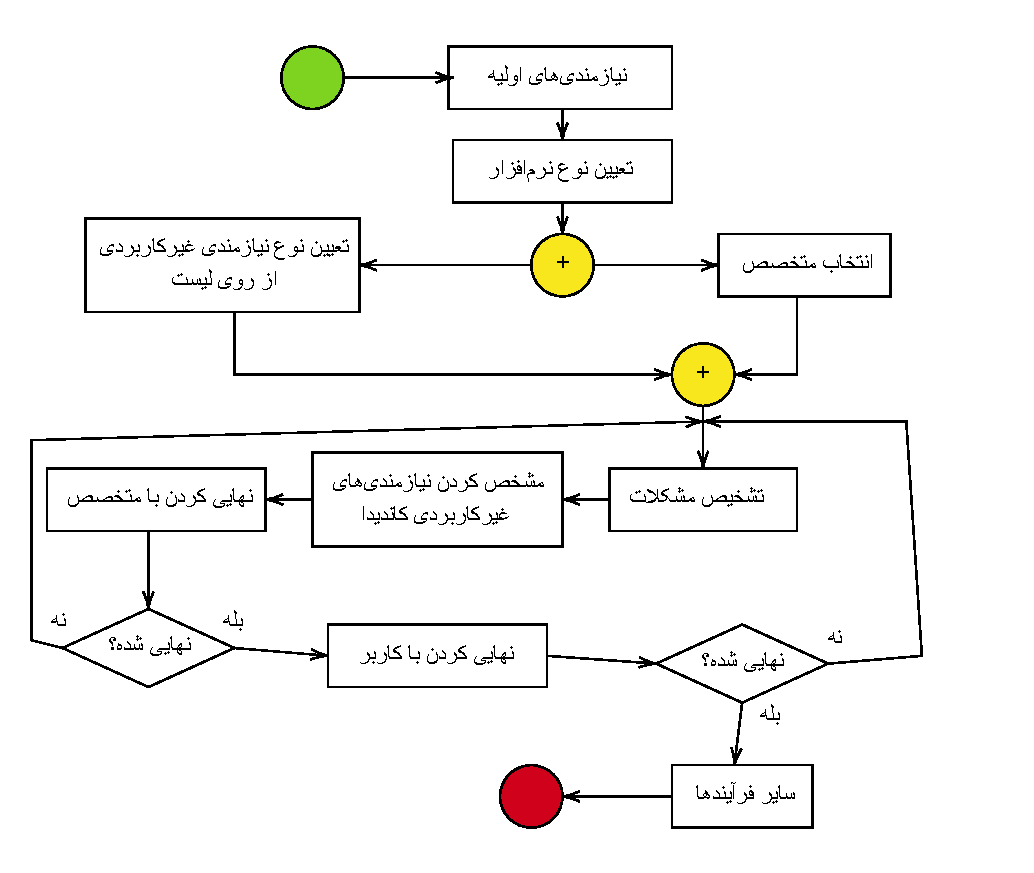
\includegraphics[scale=1.0]{figs/1-1.pdf}
	\caption{نمودار روش استخراج نیازمندی‌های غیرکاربردی در فرآیند‌های چابک \cite{guideline}}	
	\label{fig1}
\end{figure}

\end{center}
\end{enumerate}
	

\subsection*{مراجع}

\begin{latin}
	\begingroup
	\renewcommand{\section}[2]{}%
	
\begin{thebibliography}{9}
%   Check this for adding items: https://www.student.unsw.edu.au/how-do-i-cite-electronic-sources

	\bibitem{pressman}
	R. Pressman,   B. Maxim, (2014),
	\textit{Software Engineering: A Practitioner’s Approach, 8th Ed. },
	McGraw-Hill.

	
	
	\bibitem{chung}
	L. Chung,  J. Leite, (2009),
	\textit{On Non-Functional Requirements in Software Engineering},
	
	
	\bibitem{Anton}
	A. Antón, (1997),
	\textit{Goal Identification and Refinement in
	the Specification of Information Systems}. PhD Thesis,
	Georgia Institute of Technology.
	
	\bibitem{davis}
	A. Davis, (1993), \textit{Software Requirements: Objects, Functions
	and States.} Prentice Hall.

	\bibitem{Rumbaugh}
	I. Jacobson, G. Booch, and J. Rumbaugh, (1999), \textit{The
	Unified Software Development Process}, Reading,
	Mass.: Addison Wesley.
	
	\bibitem{Ncube}
	C. Ncube, (2000), \textit{A Requirements Engineering Method
	for COTS-Based Systems Development}, PhD Thesis,
	City University London.
	
	
	\bibitem{wiegers}
	K. Wiegers, (2003), \textit{Software Requirements}, 2nd edition.
	Microsoft Press.
	
	\bibitem{refqs}
	B. Paech, and D. Kerkow,  (2004), \textit{Non-Functional Requirements Engineering - Quality is Essential}.
	REFQS 2004.


	\bibitem{iso25010}
	ISO/IEC 25010, (2011),\textit{ Systems and software engineering — Systems and software Quality Requirements and Evaluation (SQuaRE) - System and software quality models}
	
		 \bibitem{elicit}
	M. Younas et al., (2010), \textit{Elicitation of Nonfunctional Requirements in Agile Development Using Cloud Computing Environment}, in IEEE Access, doi: 10.1109/ACCESS.2020.3014381.
	
	\bibitem{Teamly}
	M. Corbin,
	\textit{Catching a Cloud, Pinning it Down: How to Capture Non Functional Requirements in Agile},
	Accessed on 12/3/2022,
	\url{https://www.teamly.com/blog/how-to-capture-non-functional-requirements-in-agile/}
	
	\bibitem{lightning}
	 D. Saboe, (2019),
	 \textit{Lightning Cast: Non-Functional Requirements in Agile},
	 Accessed on 12/3/2022,
	 \url{https://masteringbusinessanalysis.com/lightning-cast-non-functional-requirements-in-agile/}
	 
	 	  

	\bibitem{guideline}
	M. Younas et al., (2017).
	\textit{Non-Functional Requirements Elicitation Guideline for Agile Methods}. Journal of Telecommunication, Electronic and Computer Engineering.
	 


	
	
\end{thebibliography}
\endgroup
\end{latin}

}
